\section{Introduction}
\label{s:lab2-introduction}
Active enumeration is when a user programmatically gather informations on a
system through the use of a set of predefined commands
\citep{cooperWhatDifferenceActive2020}. The most common set of informations that
is usually gathered through enumeration are DNS, IPs, ports, and services.

\section{Final output}
\label{s:lab2-final-output}
The software that has been written for this lab is a simple but effective nmap
clone. Once executed it asks for a range of ip addresses and then starts to ping
them incrementally starting from the first input till the end. While pinging, it
first of all recognise if the machine is responding, and it then looks for open
ports, mac addresses, dns and ttl. At the end of the scan, when the objects has
been populated, it will then produce a final report with all the information
gathered during the process. All the tools used to write the code is primitive and already
included in python. The final output of the python program can be executed
with \lstinline{python action.py}.
\begin{figure}[H]
  \centering
  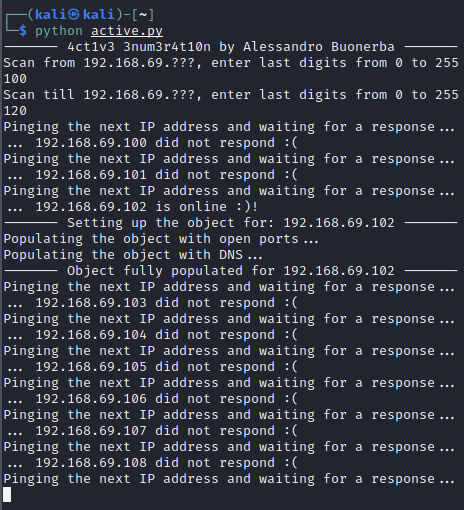
\includegraphics[width=0.4\textwidth]{figures/scrolling-text}
  \caption{Executing the Custom Nmap Clone}
  \label{f:scrolling-text}
\end{figure}
The figure above, shows how the program asks for an input by the user. In order
to know which IP to ping, it will ask for a range to scan. Once the user gives
in the requested information, it will then start to scan and print an updated of
what it is doing step by step.
Once it finishes to scan the range, it will print the final report with a list
of IPs and all the informations gathered during the previous step. At the end of
the list it will also print a nice general summary report as shown below.
\begin{figure}[H]
  \centering
  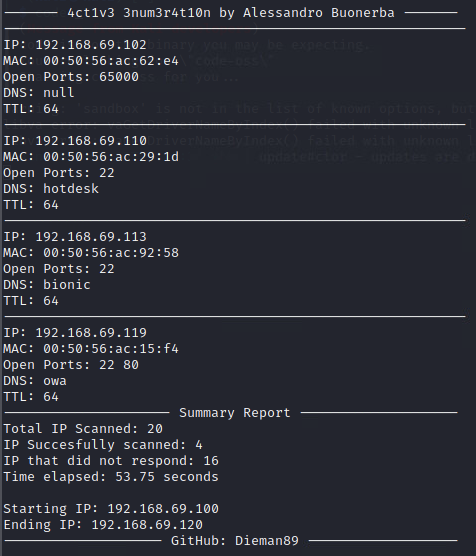
\includegraphics[width=0.5\textwidth]{figures/result-active-enum}
  \caption{Results and Summary Report}
  \label{f:result-active-enum}
\end{figure}

\section{Python Code}
\label{s:lab2-python-code}
The code has been written with primitive tooling, meaning that all the packages
imported were already installed in the VM and part of the python language. The
figure below shows the imports of the packages used to accomplish the tasks.
Here is a list of the modules used:
\begin{itemize}
  \item \lstinline{socket} provides access to the socket interface and is available on almost all modern platforms.
  \item \lstinline{os} provides acccess to the miscellaneous operating system interfaces.
  \item \lstinline{time} provides access to time-related functions.
  \item \lstinline{platform} provides access to underlying platform-s identifying data.
  \item \lstinline{subprocess} provides access to spawn processes and their input/output.
  \item \lstinline{re} provides access to regular expression matching operations.
\end{itemize}
\begin{figure}[H]
  \centering
  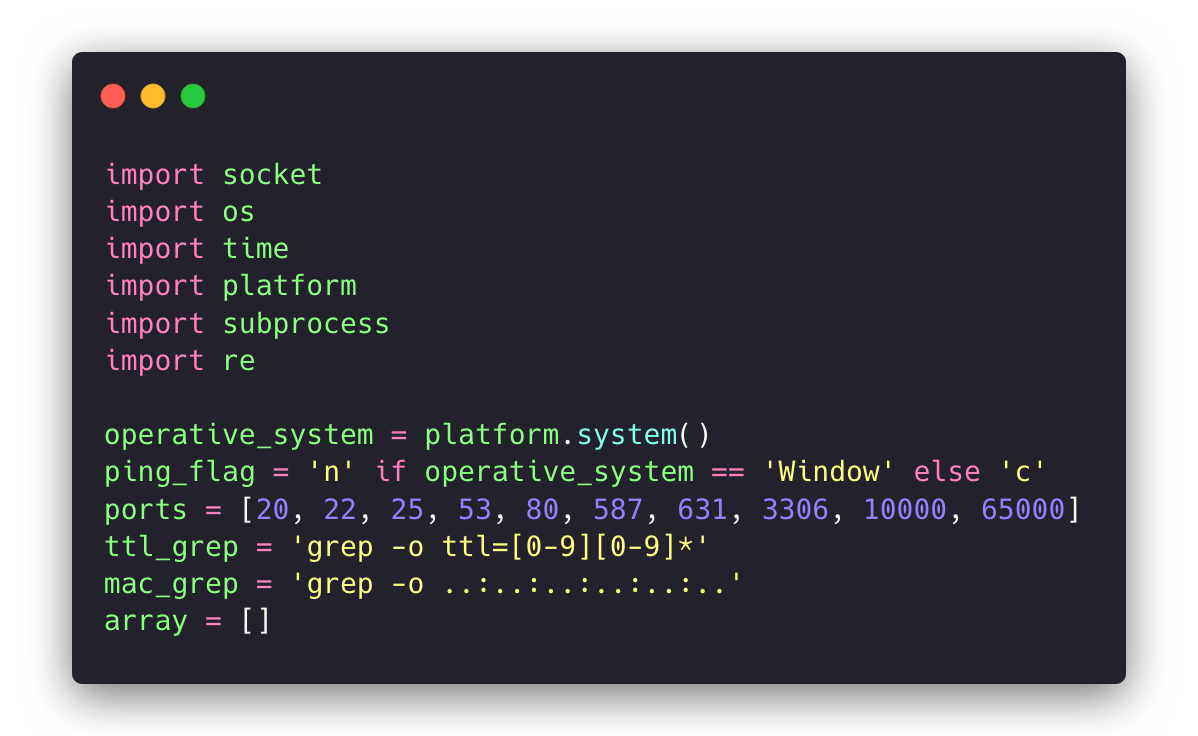
\includegraphics[width=0.7\textwidth]{figures/code/imports}
  \caption{imports-declarations}
  \label{f:imports-declarations}
\end{figure}

There are also some variables that have been set globally in order to be used
anywhere in the code. The operative system variable has been used to check
system where the code is running as the ping command would have a different flag
depending on this factor. An array of the most important ports is also declared,
where initially the first iteration of the software would scan a large set of
ports. The grep for TTL and MAC format are respectively used to extract them
from other commands. The \lstinline{ping_flag} and \lstinline{ttl_grep} are used in the main code
shown in Figure \ref{f:main}, \lstinline{ports} is used in the code in Figure
\ref{f:format-ports} while \lstinline{mac_grep} is used in the code shown in
figure \ref{f:format-arp}.

\begin{figure}[H]
  \centering
  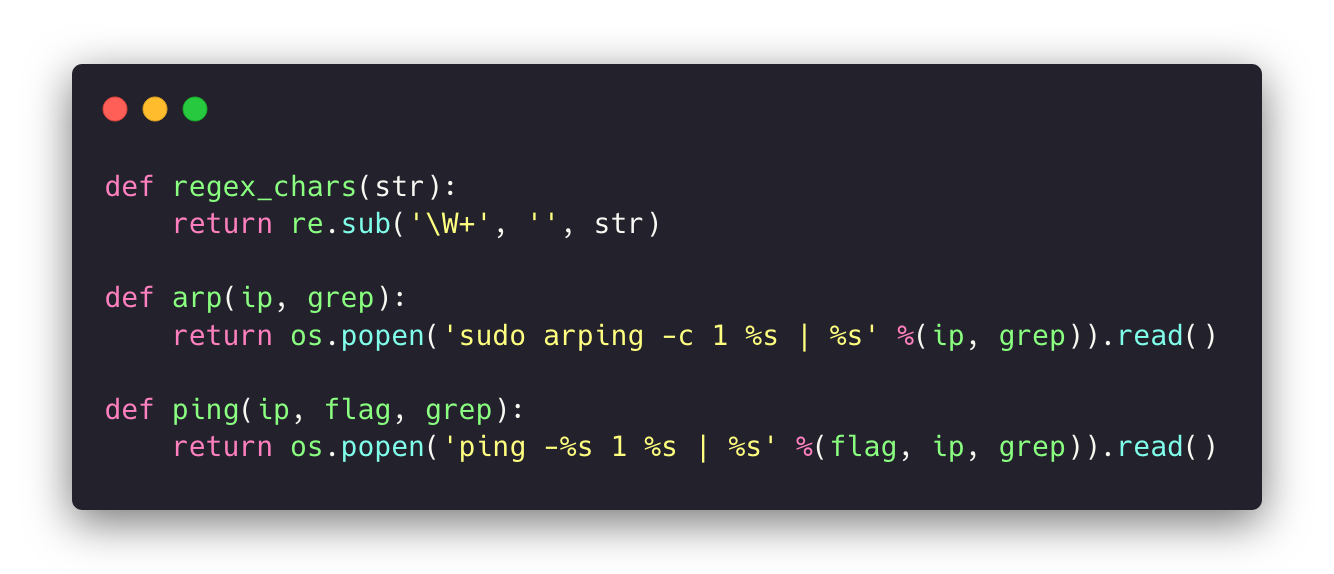
\includegraphics[width=0.7\textwidth]{figures/code/regex-arp-ping}
  \caption{Regex, arping and ping}
  \label{f:regex-arp-ping}
\end{figure}

The function \lstinline{regex_chars} takes a string as a parameter and returns a
string that gets cleaned from all the extra characters that are not letters
through regular expression. The regex function is called in the code shown in
picture \ref{f:format-dns}. The function \lstinline{arp} takes two strings as
parameters, one being \lstinline{ip} and the other being \lstinline{grep}. This
function will basically run the arping command and will be called later in the
Figure \ref{f:format-arp}. The last function \lstinline{ping} takes three
strings as arguments same as the previous one, but with the exception of the
additional flag that will injected in the command depending on which operative
system the machine is running on. Also, this function is called in the main
method shown in the Figure \ref{f:main} Since the VM has only the old Python 2.7,
the old \lstinline{%} has been used to format with a specifier to say how the
value should be go in. With Python >= 3.6, it is usually replaced with the more
flexible \lstinline{f-strings}.

\begin{figure}[H]
  \centering
  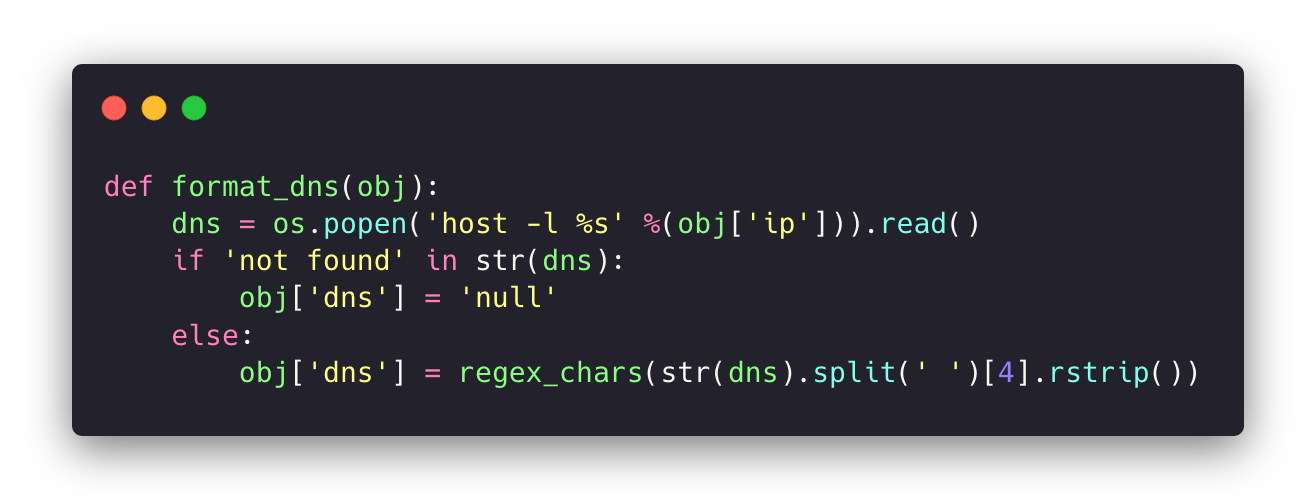
\includegraphics[width=0.7\textwidth]{figures/code/format-dns}
  \caption{Format DNS}
  \label{f:format-dns}
\end{figure}

The function \lstinline{format_dns} takes a dictionary as a parameter, where has
been created and partially populated in Figure \ref{f:format-arp}. The IP will
be the referenced key and its value used to perform the host command to find the
dns name. Since the messages are printed in terminal in a very predefined format,
the string will get splitted and transformed in an array where name of the dns
gets picked and removed from any special characters, in this case a dot and the
results gets populated in the dns key of the dictionary as a value. If the host
is not found, it will push a null value instead.
\begin{figure}[H]
  \centering
  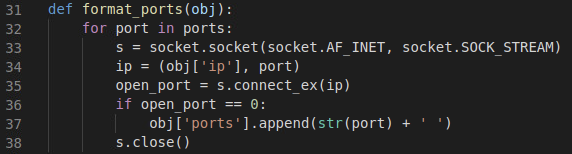
\includegraphics[width=0.7\textwidth]{figures/code/format-ports}
  \caption{Format Ports}
  \label{f:format-ports}
\end{figure}

The function \lstinline{format_ports} takes again a dictionary as parameter,
similarly to the previous one, and loops through the array ports that are
globally declared in figure \ref{f:imports-declarations}. It creates a socket
object that specify address family and socket type, respectively
\lstinline{IPv4} and \lstinline{TCP}. Moving down, an ip variable will be
created to reference the ip address and a port. This variable will then be used
as a parameter to the \lstinline{connect_ex} method from the socket object
previously created and assigned again to another variable. If the last variable
is \lstinline{0}, it means that the operation has been successfull and the port
is open. The last step is to append the open port to the dictionary after
converting it to a string.

\begin{figure}[H]
  \centering
  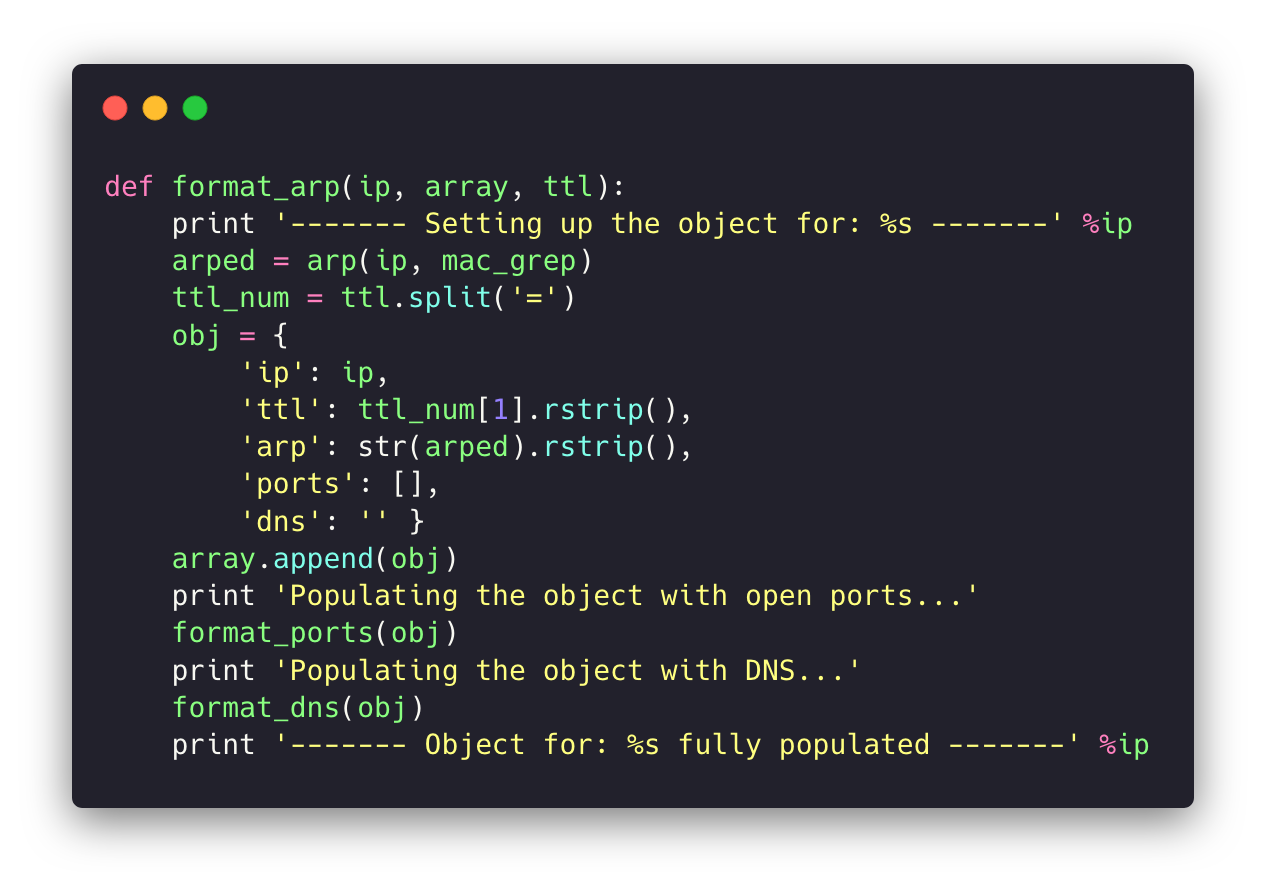
\includegraphics[width=0.7\textwidth]{figures/code/format-arp}
  \caption{Format ARP}
  \label{f:format-arp}
\end{figure}

The function \lstinline{format_arp} takes three parameters, the first one being
an ip as a string, the second one an array and a TTL format string that will be
previously grepped from the main before calling this function. This function
will initialise the object structure of each IP that will then be pushed into
the global array. It will also partially populate it with IP and TTL that will
get passed from main and ARP that will contain the MAC address generated from
the \lstinline{arp} function. The \lstinline{rstrip()} method is used to remove
the extra characters that are not needed, such as whitespaces. The object will
then be appended to the array, that will then be referenced in
\lstinline{format_ports} and \lstinline{format_dns} functions. From now on the
mutations will be done on the array level. Lastly, some print to the terminal
will be done here to keep the user updated on the progress.

\begin{figure}[H]
  \centering
  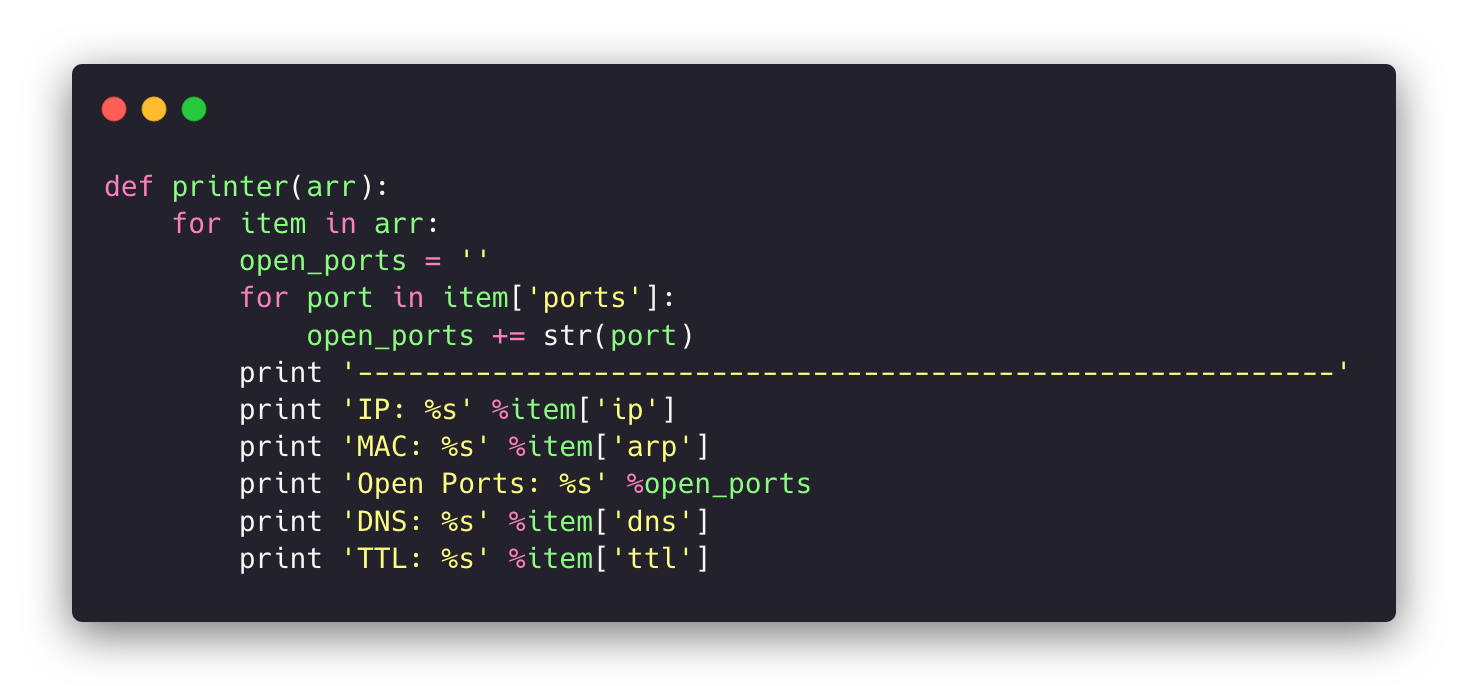
\includegraphics[width=0.7\textwidth]{figures/code/printer}
  \caption{Printer}
  \label{f:printer}
\end{figure}

The \lstinline{printer} function takes an array as a parameter. It is used
almost at the end of the main method in Figure \ref{f:main} and gives the
human-readable representation of the infromations gathered throughout the
enumeration.

\begin{figure}[H]
  \centering
  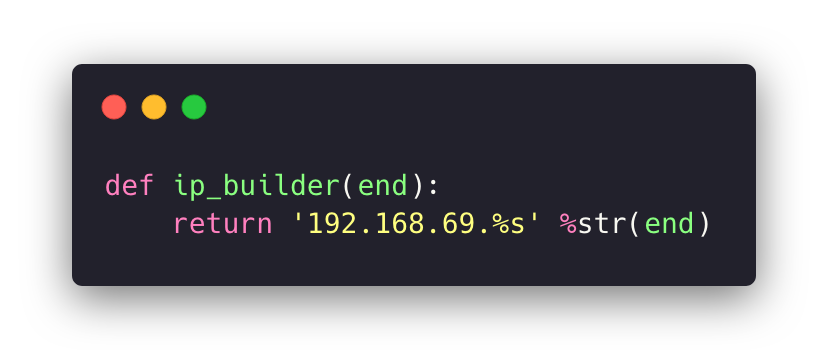
\includegraphics[width=0.7\textwidth]{figures/code/ip-builder}
  \caption{IP Builder}
  \label{f:ip-builder}
\end{figure}

This simple function is used in main before calling the function that will then
ping it. It returns the IP address that must be pinged and starts the whole
process.

\begin{figure}[H]
  \centering
  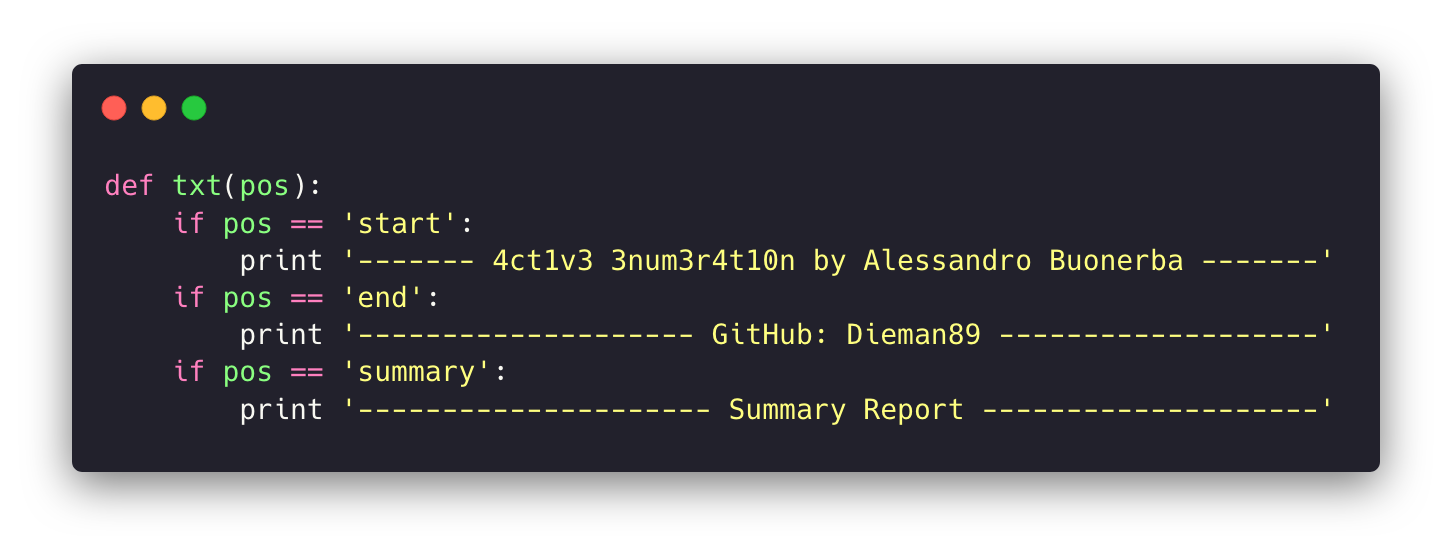
\includegraphics[width=0.7\textwidth]{figures/code/txt}
  \caption{Text Function}
  \label{f:txt}
\end{figure}

This function is used as a reference to some of the strings printed within the code.

\begin{figure}[H]
  \centering
  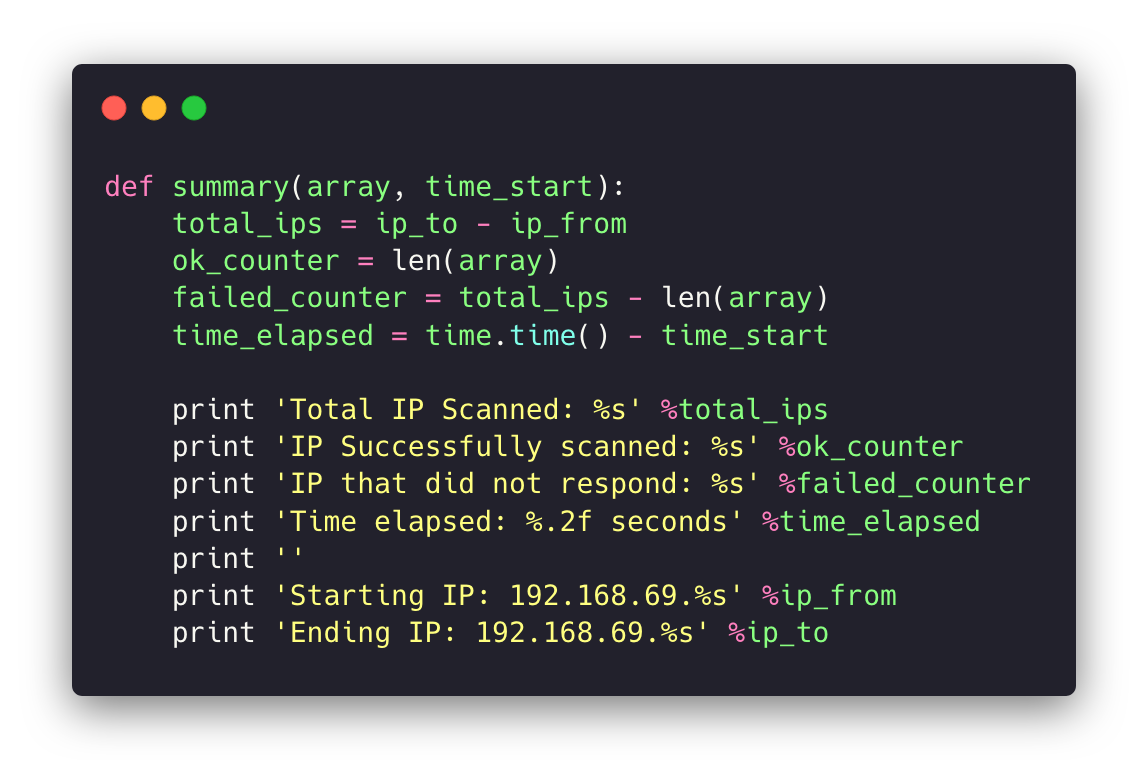
\includegraphics[width=0.7\textwidth]{figures/code/summary}
  \caption{Summary Function}
  \label{f:summary}
\end{figure}

The \lstinline{summary} function takes and array a string that stores the start
time of the program. The array is passed when the objects within it are fully
populated and is used as a reference to calculate some of the metrics such as ip
successfully and failed scanned ips. The start time, instead is passed from the
main and re-used in the function where a new time method is called to calculate
the time elapsed. At the end, all the data is printed to the user in a
human-readable way.

\begin{figure}[H]
  \centering
  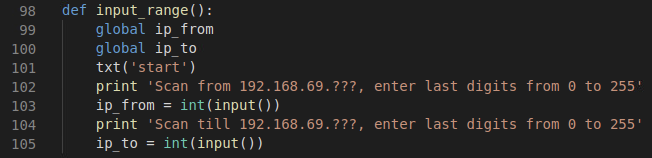
\includegraphics[width=0.7\textwidth]{figures/code/input-range}
  \caption{Input Range}
  \label{f:input-range}
\end{figure}

The function above will be called as first thing at the start of the
program in order to ask the user for the range of IPs to be scanned. It sets the
global within the methods for readability and better understanding, as they will
then be used throughout the code.

\begin{figure}[H]
  \centering
  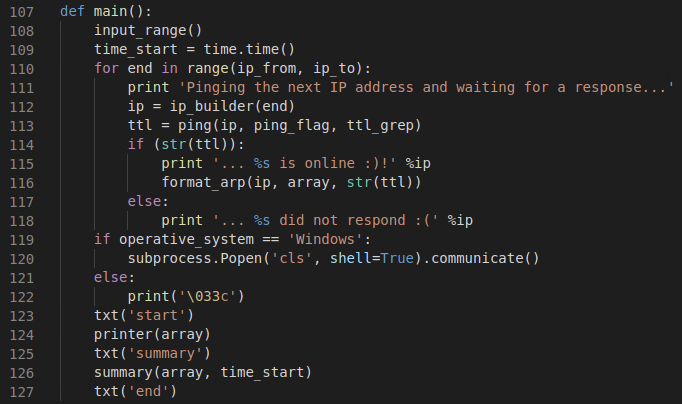
\includegraphics[width=0.7\textwidth]{figures/code/main}
  \caption{The Main}
  \label{f:main}
\end{figure}

Finally the \lstinline{main}. This has been referenced multiple times throughout
the report of this lab and probably does not need to be explained further. Few
things that are still not explained are the subprocess object with the Popen
method used to clear the terminal on Windows, and the \lstinline{print('\033c')}
used to clear the terminal on Unix. On a note, this is where a time sleep would
be implemented in order to bypass network bandwith overload as specified and
asked in one of the tasks.

\begin{figure}[H]
  \centering
  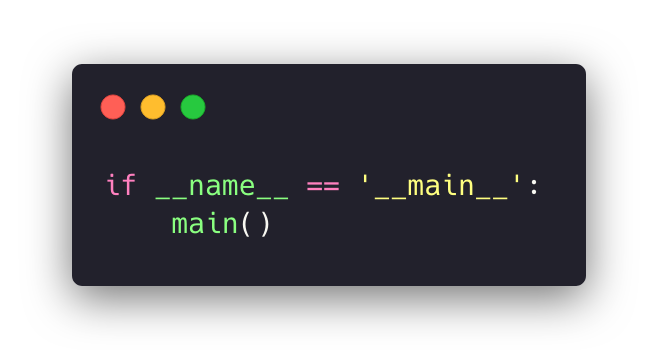
\includegraphics[width=0.7\textwidth]{figures/code/namemain}
  \caption{Name variable as main}
  \label{f:namemain}
\end{figure}

As in almost any Python code, this sets the name variable as main and then call
the main method.

\begin{figure}[H]
  \centering
  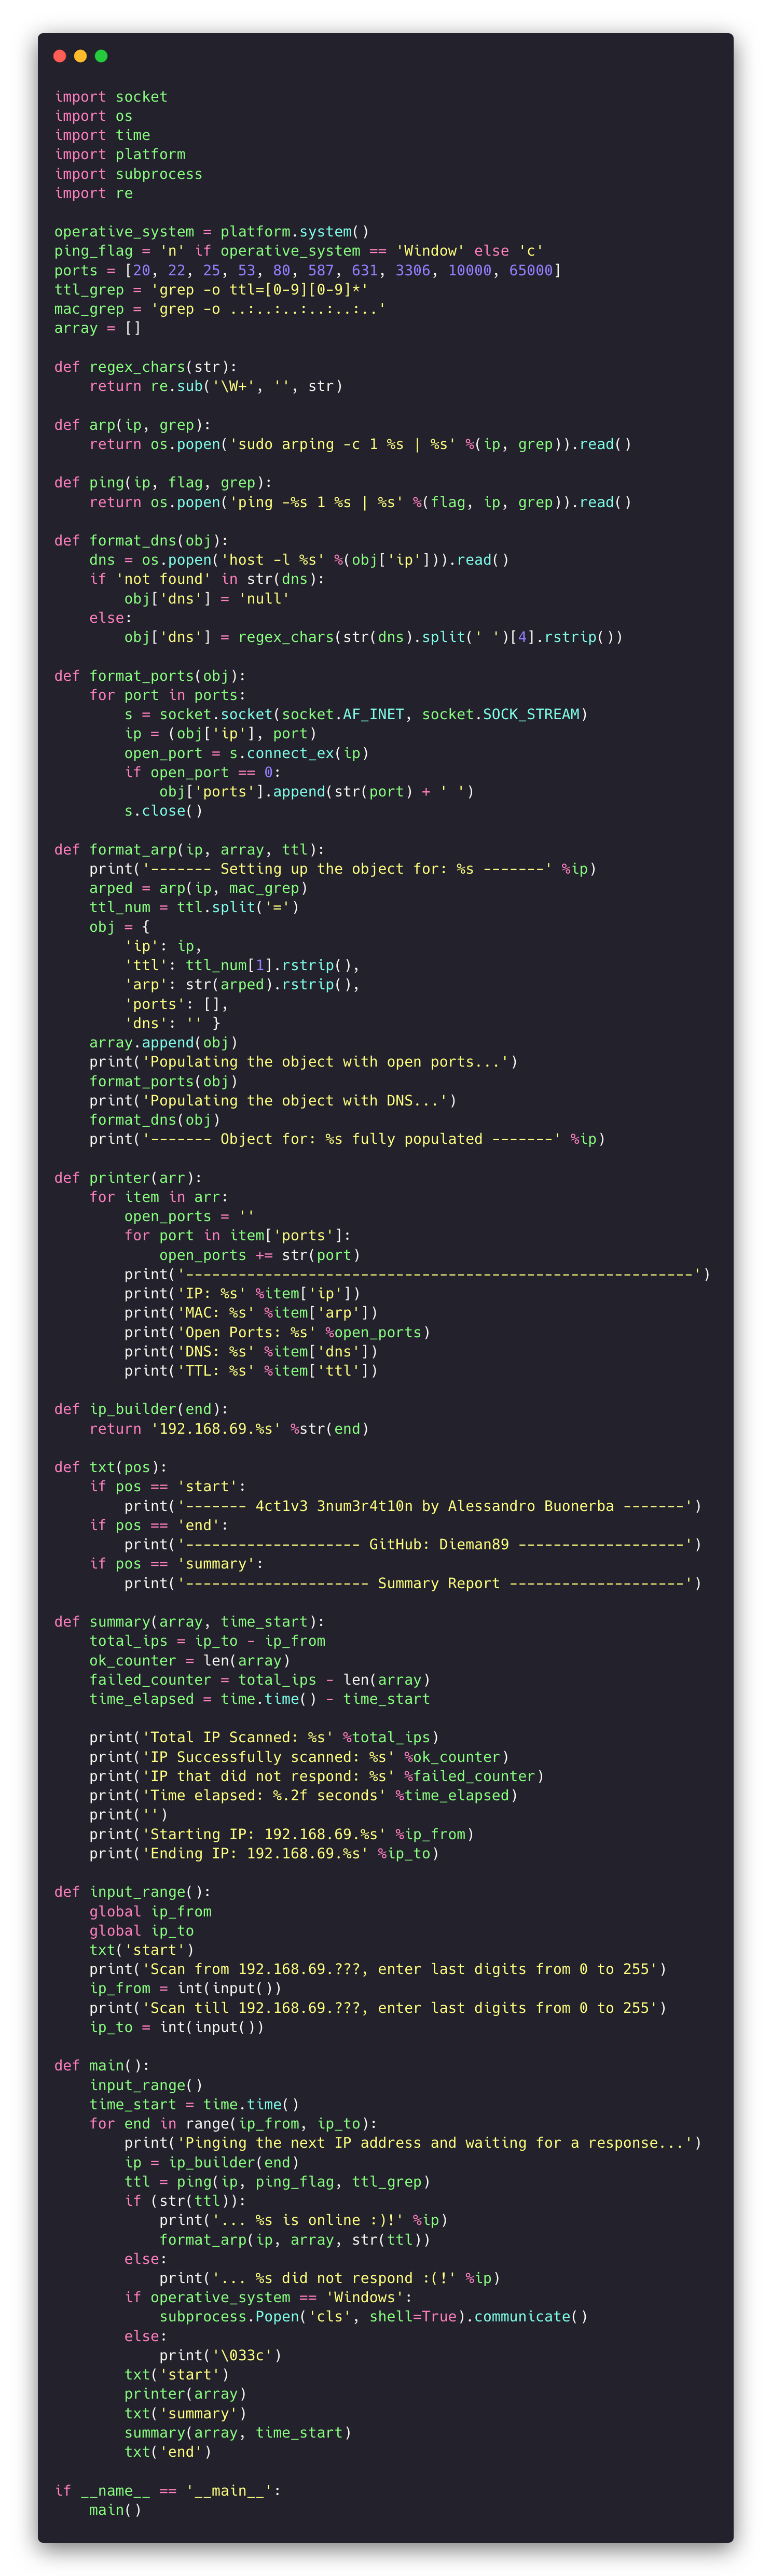
\includegraphics[width=0.4\textwidth]{figures/code/enum-full-code}
  \caption{Full Code}
  \label{f:enum-full-code}
\end{figure}
Above the full code for better readability.

\section{Conclusion}
\label{s:lab2-conclusion}
This has been one of the most fun lab I have ever done at the University. I have
learned more about active enumeration and basically created a nmap clone with
very primitive tooling. The only downside is the isolation of the machine from
internet, and the fact that is very very slow. It created a very slow and far
from good developer experience but I understand how not much can be done to fix
it. Research has been done on Python syntax as it is not my main language.
Overall a very positive experience, and I am very happy with the final product.
